
%%%%%%%%%%%%%%%%                                ~~~~~~~~~~~~~~~~~~~~~~~~~~~~~~~~~~~~~~~~~~~~~~~~~~
% CONDITIONALS %
%%%%%%%%%%%%%%%%                                ~~~~~~~~~~~~~~~~~~~~~~~~~~~~~~~~~~~~~~~~~~~~~~~~~~

\newif\ifPeerReview\PeerReviewfalse             % Whether to create the PeerReview version or
                                                % Journal version
\newif\ifFlatArchive\FlatArchivefalse           % Whether archive is flat (messy) or contain 
                                                % subfolders for graphics etc.
\newif\ifFloatAtEnd\FloatAtEndfalse             % Available in PeerReview mode:
                                                % Place floats at end of document?
\newif\ifTODO\TODOtrue                          % Use todo notes?

%%%%%%%%%%%%%%                                  ~~~~~~~~~~~~~~~~~~~~~~~~~~~~~~~~~~~~~~~~~~~~~~~~~~
% ECUA style %
%%%%%%%%%%%%%%                                  ~~~~~~~~~~~~~~~~~~~~~~~~~~~~~~~~~~~~~~~~~~~~~~~~~~

\documentclass[10pt,a4paper]{article}
\usepackage{template/ecua}

%%%%%%%%%%%%%%%%%%%%%%%%%%%%%%                  ~~~~~~~~~~~~~~~~~~~~~~~~~~~~~~~~~~~~~~~~~~~~~~~~~~
% ECUA ''APPROVED'' PACKAGES %
%%%%%%%%%%%%%%%%%%%%%%%%%%%%%%                  ~~~~~~~~~~~~~~~~~~~~~~~~~~~~~~~~~~~~~~~~~~~~~~~~~~

% load some other useful packages
\usepackage{cite} % improved formatting for citation lists
\usepackage{graphicx}

%%%%%%%%%%%%%%%%%%%%%%%                         ~~~~~~~~~~~~~~~~~~~~~~~~~~~~~~~~~~~~~~~~~~~~~~~~~~
% ADDITIONAL PACKAGES %       
%%%%%%%%%%%%%%%%%%%%%%%                         ~~~~~~~~~~~~~~~~~~~~~~~~~~~~~~~~~~~~~~~~~~~~~~~~~~

\usepackage{glossaries}
\usepackage[table,dvipsnames,svgnames]{xcolor}
\newcounter{todoidx}

\ifTODO
   \definecolor{todobackground}{rgb}{0.95,0.95,0.95}
   \setlength\marginparsep{1pt}
   \setlength\marginparwidth{35pt}
   \newlength\marginparwidthsmall
   \setlength\marginparwidthsmall{\marginparwidth}
   \addtolength\marginparwidthsmall{+6mm}
   \newcommand\todo[1]{%
      \addtocounter{todoidx}{1}%
      {\color{Red}\fbox{\bf\thetodoidx{}}}%
      \marginpar{%
         {\vspace*{-10pt}\color{Red}\fbox{\bf\thetodoidx{}}}\\%
         \fcolorbox{red}{todobackground}{\parbox{\marginparwidthsmall}{\scriptsize #1}}}}

   \newcommand\todopar[1]{\fcolorbox{red}{white}{\parbox{0.97\linewidth}{#1}}}
\else
%    \usepackage[disable]{./todonotes} 
   \newcommand\todo[1]{}
\fi

\newenvironment{narrow}[2]{%
\begin{list}{}{%
\setlength{\topsep}{0pt}%
\setlength{\leftmargin}{#1}%
\setlength{\rightmargin}{#2}%
\setlength{\listparindent}{\parindent}%
\setlength{\itemindent}{\parindent}%
\setlength{\parsep}{\parskip}}%
\item[]}{\end{list}}

\usepackage{float}

%%%%%%%%%%                                      ~~~~~~~~~~~~~~~~~~~~~~~~~~~~~~~~~~~~~~~~~~~~~~~~~~
% MACROS %       
%%%%%%%%%%                                      ~~~~~~~~~~~~~~~~~~~~~~~~~~~~~~~~~~~~~~~~~~~~~~~~~~

\newcommand\Eq[1]{Equation (\ref{#1})}
\newcommand\Fig[1]{Figure \ref{#1}}

\newcommand\Grey[1]{{\color{Grey}#1}}
\newcommand\Red[1]{{\color{Red}#1}}
\newcommand\Blue[1]{{\color{Blue}#1}}
\newcommand\DarkBlue[1]{{\color{DarkBlue}#1}}
\newcommand\LightBlue[1]{{\color{LightBlue}#1}}
\newcommand\Brown[1]{{\color{Brown}#1}}
\newcommand\Green[1]{{\color{Green}#1}}
\newcommand\SeaGreen[1]{{\color{SeaGreen}#1}}
\newcommand\Yellow[1]{{\color{yellow}#1}}
\newcommand\Orange[1]{{\color{orange}#1}}

\newcommand\nn{\nonumber\\}

\newcommand\nmat[1]{\begin{matrix}#1\end{matrix}}
\newcommand\bmat[1]{\begin{bmatrix}#1\end{bmatrix}}
\newcommand\case[1]{\begin{cases}#1\end{cases}}
\newcommand\textbox[2]{\footnotesize\text{\parbox{#1}{\centering\emph{#2}}}}

\newcommand\rand{\text{rand}}
\newcommand\randn{\text{randn}}
\newcommand\rect{\text{rect}}
\newcommand\sinc{\text{sinc}}
\newcommand\tr{\text{tr}}
\newcommand\adj{\text{adj}}

% \newcommand\max{\text{max}}
\newcommand\argmin{\text{argmin}}

\newcommand\qqquad{\quad\qquad}
\newcommand\qqqquad{\qquad\qquad}

\renewcommand\l[1]{\left#1}
\renewcommand\r[1]{\right#1}

% {\text{\parbox{1.5cm}{\centering volume hyper- sphere}}}

%Keyword colouring:
\newcommand\kw[1]{#1}
\newcommand\parm[1]{#1}%\color{Black}#1\color{Black}}

\newcommand\of[1]{\scriptstyle(\parm{#1})\displaystyle}
\newcommand\df[1]{\scriptstyle[\parm{#1}]\displaystyle}
\newcommand\var[3]{#1_\text{#2}\of{#3}}

\newcommand\diag{\text{diag}}

% \raisebox{lift}[extend-above-baseline][extend-below-baseline]{text}
\newcommand\mt[1]{\text{\emph{#1}}} %mt = mathtext
\newcommand\mathnorm{\textstyle}
\newcommand\mathbig[1]{\displaystyle#1\mathnorm}
\newcommand\mathsmall[1]{\scriptstyle#1\mathnorm}
\newcommand\mathtiny[1]{\scriptscriptstyle#1\mathnorm}
\newcommand\sfrac[2]{\scriptstyle\raisebox{0.25pt}[0pt][0pt]{$\frac{#1}{#2}$}\mathnorm}
\newcommand\nfrac[2]{\textstyle\frac{#1}{#2}\displaystyle}

\newcommand\sumu[1]{\sum\limits^{#1}\,}
\newcommand\suml[1]{\sum\limits_{#1}\,}
\newcommand\sumb[2]{\sum\limits_{#1}^{#2}\,}

\newcommand\produ[1]{\prod\limits^{#1}\,}
\newcommand\prodl[1]{\prod\limits_{#1}\,}
\newcommand\prodb[2]{\prod\limits_{#1}^{#2}\,}

\newcommand\defeq{\overset{\underset{\mathrm{def}}{}}{=}}

%Math macros:
\newcommand\diff[2]{\frac{\kw{d}\,\textstyle #1\scriptstyle}{\kw{d\parm{#2}}}\displaystyle}
\newcommand\ddiff[2]{\frac{\kw{d^2}\,\displaystyle #1\scriptstyle}{\kw{d\parm{#2}}^2}\displaystyle}

\renewcommand\d[1]{\scriptstyle\kw{\,d\parm{#1}}\displaystyle}

% These commands are mutually exclusive. Remember to "renew" in v2.
\newcommand\intb[4]{\int\limits_{#3}^{#4} #1 \d{#2}} % \int{exp}{var}{from}{to}
\newcommand\intl[3]{\int\limits_{#3} #1 \d{#2}} % \int{exp}{var}{for all}
\newcommand\intu[2]{\int #1 \d{#2}} % \int{exp}{var}{for all}

\newcommand\T{^{\scriptscriptstyle T}}
\renewcommand\H{^{\scriptscriptstyle H}}

\renewcommand\vec[1]{\boldsymbol{#1}}
\newcommand\mat[1]{\boldsymbol{#1}}

\newcommand\1{\vec 1}
\newcommand\I{\mat I}
\renewcommand*\a{\vec a}
\renewcommand*\i{\vec i}
\renewcommand*\k{\vec k}
\newcommand*\n{\vec n}
\newcommand*\p{\vec p}
\newcommand*\s{\vec s}
\newcommand*\w{\vec w}
\newcommand*\x{\vec x}
\newcommand*\y{\vec y}

\newcommand*\A{\mat A}
\newcommand*\B{\mat B}
\newcommand*\C{\mat C}
\newcommand*\E{\mat E}
% \renewcommand*\H{\mat H}
\renewcommand*\P{\mat P}
\newcommand*\eP{\mat{\hat P}}
\newcommand*\R{\mat R}
\newcommand*\Ri{\R^{-1}}
\newcommand*\eR{\mat{\hat R}}
\newcommand*\eRi{\hat{\mat R}\,\!^{-1}}
\newcommand*\Navg{N_\text{avg}}
\newcommand*\W{\mat W}
\newcommand*\X{\mat X}
\newcommand*\Xd{\X_{\!\Delta}}
\newcommand*\Y{\mat Y}

\renewcommand*\L{\mat \Lambda}
\newcommand*\U{\mat U}
% \renewcommand*\t{\mathtiny{^T}}
% \newcommand*\h{\mathtiny{^H}}
\renewcommand*\t{^T}
\newcommand*\h{^H}

\newcommand\D{\vec\nabla} %Del: Vector differential operator - nabla
\newcommand\Dx{\vec\nabla\times}
\newcommand\Dd{\vec\nabla\cdot}

% \usepackage{tikz}
% \usetikzlibrary{shapes,snakes}
\usepackage{amsmath,amssymb}

\newenvironment{outline}
{\begin{itemize}}
{\end{itemize}}

%    \definecolor{todobackground}{rgb}{0.95,0.95,0.95}
%    \setlength\marginparsep{3pt}
%    \setlength\marginparwidth{42pt}
%    \newlength\marginparwidthsmall
%    \setlength\marginparwidthsmall{\marginparwidth}
%    \addtolength\marginparwidthsmall{-7pt}
%    \newcommand\todo[1]{%
%       \addtocounter{todoidx}{1}%
%       {\color{Red}\fbox{\bf\thetodoidx{}}}%
%       \marginpar{%
%          {\vspace*{-10pt}\color{Red}\fbox{\bf\thetodoidx{}}}\\%
%          \fcolorbox{red}{todobackground}{\parbox{\marginparwidthsmall}{#1}}}}
% 

% correct bad hyphenation here
% \hyphenation{op-tical net-works semi-conduc-tor}

%%%%%%%%%%%%                                    ~~~~~~~~~~~~~~~~~~~~~~~~~~~~~~~~~~~~~~~~~~~~~~~~~~
% GLOSSARY %
%%%%%%%%%%%%                                    ~~~~~~~~~~~~~~~~~~~~~~~~~~~~~~~~~~~~~~~~~~~~~~~~~~

\makeglossaries
\newglossaryentry{ASIC}{name={ASIC},
                  description={Application Specific Integrated Circuit} } 
                  
\newglossaryentry{ATR}{name={ATR},
                  description={Automatic Target Recognition} } 

\newglossaryentry{CPU}{name={CPU},
						description={Central Processing Unit} } 

\newglossaryentry{GPGPU}{name={GPGPU},
						description={General Purpose Graphics Processing Unit} } 

\newglossaryentry{GPU}{name={GPU},
						description={Graphics Processing Unit} } 
					
\newglossaryentry{MVDR}{name={MVDR},
						description={Minimum Variance Distortionless Response} } 
% windows hack for JP
% \renewcommand\gls[1]{#1}


%%%%%%%%%%%%%%%%%%                              ~~~~~~~~~~~~~~~~~~~~~~~~~~~~~~~~~~~~~~~~~~~~~~~~~~
% DOCUMENT START %
%%%%%%%%%%%%%%%%%%                              ~~~~~~~~~~~~~~~~~~~~~~~~~~~~~~~~~~~~~~~~~~~~~~~~~~


\title{GPU-based Adaptive Beamforming for Active Sonar Imaging}

\author{%
\begin{tabular}{p{45mm}p{125mm}}
Jo~Inge~Buskenes & Department of Informatics, University of Oslo, Norway \\
Jon~Petter~Aasen & Mi Lab, Norwegian University of Science and Technology, Norway \\
Carl-Inge~Colombo~Nilsen & Department of Informatics, University of Oslo, Norway \\
Andreas-Austeng & Department of Informatics, University of Oslo, Norway
\end{tabular}
}

\begin{document}


\section*{Abstract}

Two limiting factors of modern phased array sonar imaging systems are the angular resolution and contrast. Adaptive beamformers target these limitatitons by weighting sensors dynamically to fit the impinging wavefield.

The Minimum Variance (MV) adaptive beamformer has recently been introduced in active sonar imaging. While displaying great potential for creating high quality images, it is computationally intensive and relies on robustification. These are important reasons why the MV beamformer is not in widespread use today.

We propose means for adapting the MV beamformer and its robustification techniques to fit a modern Graphics Processing Unit (GPU) architecture. These devices have in recent years
emerged as a flexible and highly potent parallel technology well suited for many DSP tasks, and are available off-the-shelf at reasonable prices.

We benchmarked optimized implementations of the MV beamformer in Matlab and C, running on a quad-core Intel Xeon E5620, and in CUDA running on a mid-range nVidia card. The beamformers operated on data from the 32x4 element Kongsberg Martime HISAS1030 sonar, using a conservative set of robustification parameters. We found that the GPU rendered more than 1Mpixels/s, representing a speedup of more than two orders of magnitude over C, and three orders of magnitude over Matlab. If the HISAS1030 was attached to a platform traveling at 1.8m/s, creating full-coverage sectorscan images in realtime would be possible with this performance. The CPU would then be free to take on the rest of the beamforming as well.



\newpage
\maketitle

\section{Introduction}

% Images from a phased array active sonar system are formed in the post-processing by focusing on one pixel at a time. This is achieved by delaying and weighting each of the array's channels, providing coarse and fine adjustments to the region of focus, respectively. This is commonly referred to as beamforming. Assuming far-field conditions, the delays are usually chosen to steer the pixel of interest to broadside, and the weights chosen to reject the noise impinging on the array from non-broadside directions.
% 
% The algorithm responsible for carrying out this task is referred to as a beamformer. Depending on whether data is evaluated when choosing a suitable set of delays and weights, beamformers can be branded either conventional or adaptive. A good example of the former is the The Delay-and-Sum (DAS) beamformer, which - as the name implies - simply delay the sensor channels appropriately prior to summing them up. Applying various weight sets, or windows, to the data prior to summation allows the lateral \gls{SNR} to be improved, but at the inevitable expense of a deteriorated lateral resolution. \todo{aka. the curse of physics.}
% 
% The Minimum Variance Distortionless Response (MVDR) (or \gls{MVDR}) beamformer, have the potential to overcome this limitation. While ensuring unit gain in the look direction, it computes the set of weights that minimizes the energy accumulated by the array from other directions. In other words, whenever the distribution of noise and interference is primarily focused around specific angles, an array response with a high degree of suppression at these angles are chosen, resulting in an image with a lateral \gls{SNR} and resolution superior to anything the \gls{DAS} can come up with.

In a typical active sonar imaging scenario encoded signals are transmitted towards a surface of interest, and the resulting reflections are recorded using an array of receivers. The receiver outputs are then coherently combined in the post-processing to focus on specific points in the image. This involves assigning suitable delays and weights to the array's channels, a concept commonly referred to as beamforming.

In conventional beamforming the array sensors are assigned a static set of weights. This allows lateral resolution to be traded for improved noise suppression (contrast), but one always ends up with a compromise between the two. Adaptive beamformers target this limitation by allowing the weights to change to better fit the dynamic nature of the incoming wavefield.

The Minimum Variance Distortionless Response (MVDR, or Capon) beamformer is one such technique. While ensuring unit gain in the look direction, it computes the set of weights that minimizes the power accumulated by the array from other directions. Its ability to suppress interference power and improve image quality in active sonar systems has been demonstrated in e.g.~\cite{Blomberg2012a,Blomberg2011,Dursun2009,Lo2004}.

However, despite its inherent potential, the \gls{MVDR} beamformer has yet to see widespread adoption in the active sonar community. There may be several reasons for this. For one, the method is not inherently robust, and will suffer from a phenomenon called signal cancellation in active systems. Another reason is that in its original form, the computational complexity is cubic with the number of channels, O(M$^3$), while conventional beamformers are at O($M$).

We will show that the suggested means for making the \gls{MVDR} behave well in active systems will also make it less computationally complex. Furthermore, by implementing it on a modern \gls{GPU} we have gained a speedup of around 2 orders of magnitude compared to an optimized single-thread implementation in C.

% Yay or nay? $\Rightarrow$ GPU ultrasound (\cite{So2011,Chen2011}). Complex data, all robustification techniques.



\newpage
\section{Methods}\label{methods}

The fundamental task of sonar imaging is to estimate each pixel's individual contribution to the final recorded echo. If the data is digitally stored, we can do this by focusing on one pixel at a time in the post-processing. Since the geometric relationship of the array and image is known, one usually start by selecting delays that compensates for the difference in transmitter-pixel-receiver propagation time.

Consider an $M$ element phased array. Let the sample recorded by the $m$'th channel at time instant $n$ be represented as $x_m[n]$, and the accompanying weights be  $w_m[n]$ and $\Delta_m[n]$. To simplify the upcoming notation, let sample $x_m[n]$ delayed by $\Delta_m[n]$ be written as:
\begin{align}
x^\Delta_m = x_m[n-\Delta_m[n]].
\end{align}
The beamformer output $z[n]$ is then simply the weighted sum of all the delayed data samples:
\begin{align}
z[n] = \w\H[n]\x[n] = \bmat{w_0[n]\\w_1[n]\\\vdots\\w_{M-1}[n]}^H \bmat{x^\Delta_0[n]\\x^\Delta_1[n]\\\vdots\\x^\Delta_{M-1}[n]}.\label{z}
\end{align}
If the weights in (\ref{z}) were static, this would be referred to as the \gls{DAS} beamformer. The \gls{MVDR} beamformer~\cite{Capon1969}, however, finds the set of weights that minimizes the output power, $\min E\{|z[n]|^2\}$, while ensuring unity gain in the look direction. The solution to this optimization problem is given as:
\begin{gather}
\vec w[n] = \frac{\Ri[n]\1}{\1\T\Ri[n]\1},\label{weights}
\end{gather}
where $\1$ is a row vector of ones that represents broadside steering, and $\R=E\{\x[n]\x[n]\H\}$ is the spatial covariance matrix. Since $\R$ is unknown, it must be estimated. We will do this by computing the sample covariance matrix, $\eR$. In this computation we will perform some degree of \emph{spatial averaging} to avoid signal cancellation, \emph{temporal averaging} to achieve \gls{DAS}-like speckle statistics, and \emph{diagonal loading} to ensure a numerically well conditioned $\eR$~\cite{Synnevag2009a}.

\emph{Spatial averaging} is achieved by grouping the array channels into $M-L+1$ subarrays of length $L$, where all but one element overlap. If we let $x_l[n]$ represent the datavector from subarray $l$,
\begin{gather}
\x_l[n] = \bmat{x^\Delta_l[n] & x^\Delta_{l+1}[n] & \dots & x^\Delta_{l+L-1}[n]}\T,
\end{gather}
then the ``subarray averaged'' sample covariance matrix, $\eR_\text{s}$, is given as:
\begin{gather}
\eR_\text{s}[n] = \frac{1}{M-L+1} \sumb{l=0}{M-L} \x_l[n]\x_l\H[n].\label{spatialR}
\end{gather}

\emph{Temporal averaging} can now be introduced by taking the average of $2N_\text{avg}+1$ temporal samples of $\eR_\text{s}[n]$. Let the result be called $\eR_\text{t,s}[n]$,
\begin{gather}
\eR_\text{t,s}[n] = \frac{1}{2N_\text{avg}+1} \sumb{n'=n-N_\text{avg}}{n+N_\text{avg}} \eR_\text{s}[n'].
\end{gather}
Finally, to ensure a well conditioned sample covariance matrix, we add a fraction $d$ of the total power of $\eR_\text{t,s}[n]$ to its diagonal\cite{Synnevag2007}:
\begin{align}
\eR[n] = \eR_\text{t,s}[n] + \I \cdot \frac{d}{L} \cdot \tr\{\eR_\text{t,s}[n]\},\label{finalR}
\end{align}
where $\I$ is an identity matrix and $\tr\{\cdot\}$ means matrix trace operation.


\newpage
\section{Implementation}

Because each pixel in the image can be processed independently, the \gls{MVDR} beamformer is well suited for parallel acceleration. A technology of particular interest here are \glspl{GPU}~\cite{Nilsen2009}, which are tailored for image processing, available off-the-shelf at reasonable prices, and are found in most desktop computers already. The \gls{GPU} is a hardware architecture comprised of several hundred computing cores, each running a thread that executes a copy of a common function called a kernel.  However, there are some inherent drawbacks with such a design: Each core is left with a rather limited amount of local memory, and distributing data to the computing cores and collecting the result is a process with some inherent latency.

This suggests that the algorithm should be decomposed into as many lightweight threads as possible, which are both computationally intensive and light on the memory access and consumption. However, for a typical array configuration, using a single thread per pixel is not lightweight enough. Therefore, the methods presented section \ref{methods} had to be decomposed further. In particular, the solutions we came up with for the different steps in the algorithm, listed in their natural order of execution, was:
\begin{enumerate}
\item \emph{Computing the spatial covariance matrix} $\eR[n]$ (\ref{spatialR}-\ref{finalR}). A group of threads are created that slide along the diagonals of $\eR$. In this way we exploited the fact that entries on the diagonals overlap across subarrays and time, and keep the numbers of both data reads and writes at a minimum.
%Finished threads can also wrap around and start on diagonals on the lower half triangular. 
% In this way we process one row of $\eR$ per kernel iteration, and manage to keep the numbers of both data reads and writes at a minimum.
\item \emph{Computing} $\eRi[n]\1$ (from (\ref{weights})). While intuition may suggest that this step is carried out by inverting $\eR$, it is better to solve the linear equation $\R\beta = \1$ for $\beta$ instead, which gives us $\beta = \eRi\1$ directly. We have tested various solvers for this task, both in-house and proprietary implementations, and achieved the best performance by using an unofficial batch solver from nVidia. Inverting $\eR$ is by far the most computationally intensive task, and a key area of focus for further improvements.
\item \emph{Computing the beamformer output} $z[n]$ by substituting $\beta = \eRi[n]\1$ into (\ref{weights}), and (\ref{weights}) into (\ref{z}). A group of $L$ threads per pixel was used to reduce local memory pressure and to obtain coalesced reads and a minimum of writes. When applying weights, there are two approaches from an implementation point of view. The subarray data can, as here, be reduced to coincide in length with the subarray weights, or the weights can be extended to $M$ in size and applied directly on $\x[n]$ and summed.  
\end{enumerate}

In the upcoming results, we have beamformed pre-delayed data. This is a large dataset, and the latency experienced when copying it from the \gls{CPU} side to the \gls{GPU} was significant. However, in a practical system only the channel data should be transferred as the delaying of data can effortlessly be performed by the \gls{GPU}. The remaining latency can be hidden as long as the \gls{GPU} is kept busy, hence the data transfer times will not be reported in the upcoming results.

In this paper we have targeted an nVidia \gls{GPU} using the C interface to nVidia's \gls{CUDA} framework~\cite{NvidiaCuda}.

\begin{figure}[!t]
\centering
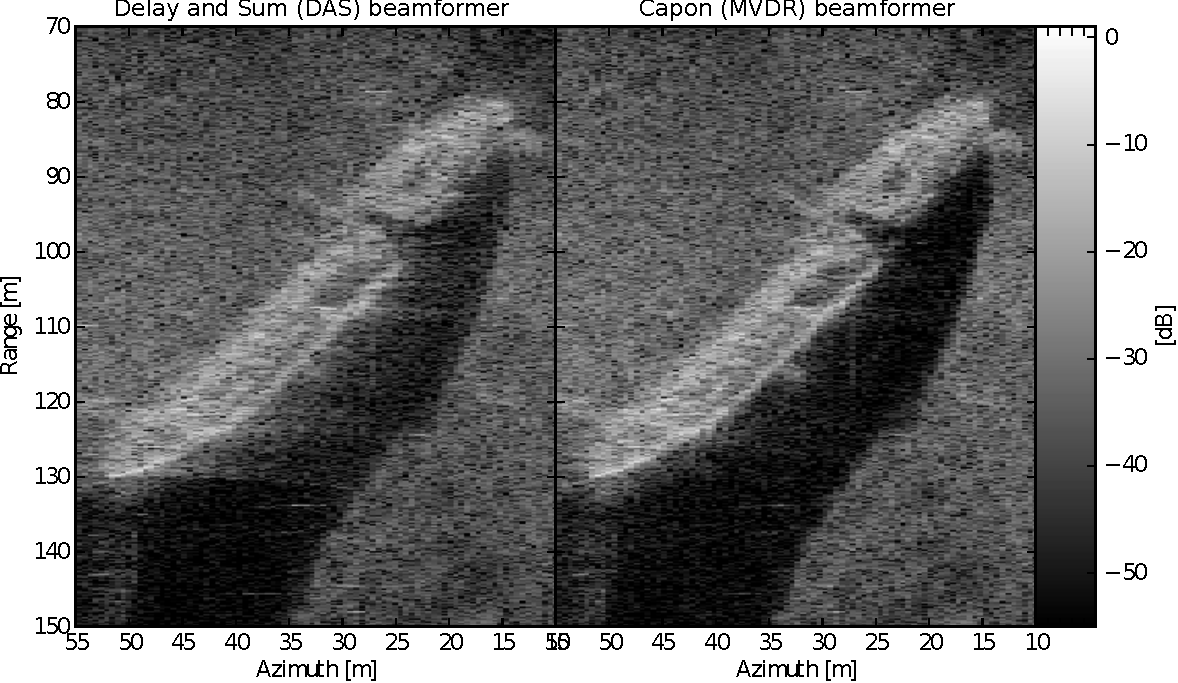
\includegraphics[width=\linewidth]{gfx/img_holmengraa.pdf}
\caption{HISAS sidescan sonar (SSS) image of the shipwreck Holmengraa.}\label{holmengraa}
\end{figure}


\newpage
\section{Results}

We have tested our \gls{GPU} implementation of the \gls{MVDR} beamformer on two different experimental datasets from the 32 element Kongsberg Maritime HISAS1030 sonar~\cite{Hansen2009}. The sonar was attached to the HUGIN \gls{AUV}, and one one of the datasets used in sidescan mode to image the 1500 dwt oil tanker wreck Holmengraa (\Fig{holmengraa}). Holmengraa is roughly 68\,m long and 9\,m wide, and lies on a slanted seabed at 77\,m depth. The \gls{MVDR} image was created with the parameters $L=16$, $N_\text{avg}=3$, and $d=1\%$, which proved to be a reasonable selection for this scenario.

\begin{figure}[!t]
\centering
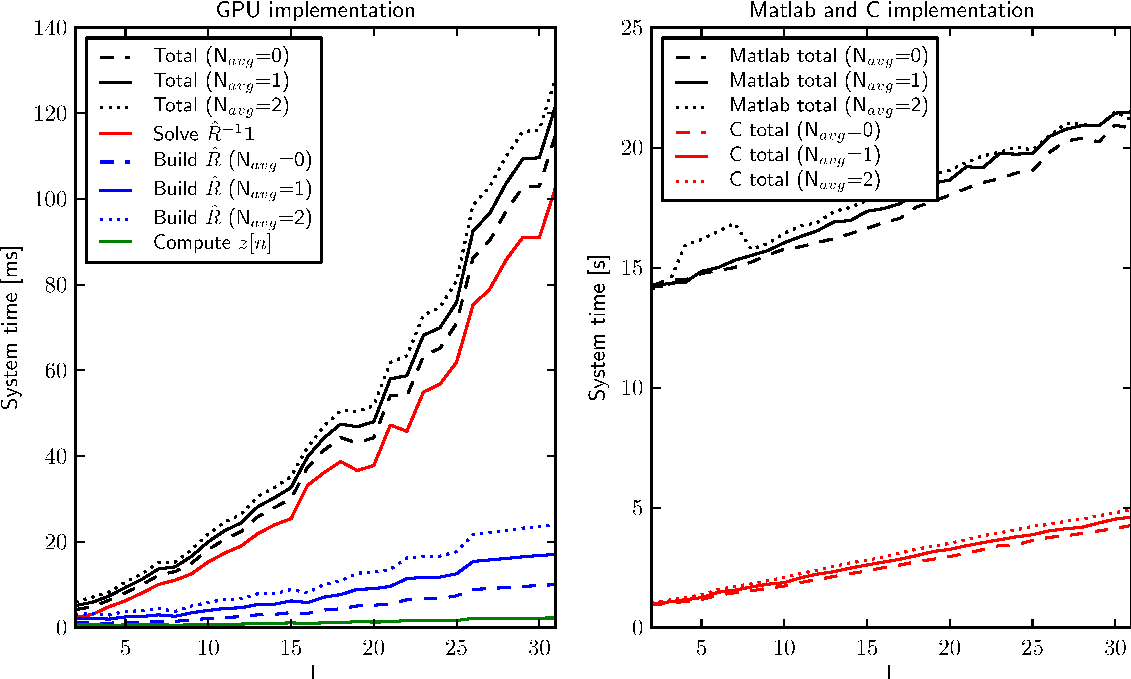
\includegraphics[width=\linewidth]{gfx/benchmark.pdf}
\caption{\gls{MVDR} benchmarks. Forming a 55\,kpixel image from a $M=32$ channel array.}\label{benchmarks}
\end{figure}

The other dataset was a 55\,kpixel sectorscan test image. We used it to benchmark our \gls{MVDR} implementation, and compared the result with the runtimes of an optimized single-thread C and Matlab implementation (\Fig{benchmarks}). Processing times are shown for varying subarray lengths $L$ and varying amounts of temporal averaging $N_\text{avg}$. The test system was a quad-core Intel Xeon E5620, with 64Gb of \gls{RAM}, and an nVidia Quadro 6000 card. This is a \gls{GPU} with 448 \gls{CUDA} cores and 6Gb of onboard \gls{RAM}, capable of performing roughly 1Tflops.

\section{Discussion}

Figure \ref{holmengraa} demonstrates the \gls{MVDR} beamformer's ability to suppress interference and achieve better detail resolution. Compared the \gls{DAS} beamformer, the ship's edges come out as sharper, and the shadows are less noisy. But while \gls{DAS} processed this 1.3\,Mpixel image in milliseconds, our Matlab implementation of \gls{MVDR} beamformer needed minutes.

As Figure \ref{benchmarks} illustrates, using a \gls{GPU} improves matters. If we look at the total runtimes for a subarray size of $L=16$ and $2N_\text{avg}+1=5$ pixels of temporal averaging, the \gls{GPU} implementation is able to process the test image in roughly 40\,ms. This translates to a processing throughput of 1.4\,Mpixels/s. For the same scenario the C implementation clocked in at roughly 3\,s and Matlab at 17\,s, which is 75 and 435 times slower than the \gls{GPU} implementation, respectively.

\newpage
Interesting to note is also that solving $\eRi\1$ remains the main bottleneck in the \gls{GPU} implementation, and it gets even worse for larger $L$'s. However, this is a general Gauss Jordan solver which does not exploit symmetry properties of $\eR$, so creating e.g.\ a batch based Cholesky solver should improve the runtimes further. Both the C and Matlab implementation in this benchmark take this symmetry into account, which partially explains why the complexity curves of these implementations are different from that of the \gls{GPU} implementation.

If the HISAS1030 was attached to a platform moving at 1.8m/s, for which the maximum range is 250\,m~\cite{Hansen2010}, the pulse repetition frequency could be set to 3\,Hz. We further assume a critical complex sampling frequency equal to the HISAS1030's bandwidth of 30\,kHz, and beamform $M=32$ lateral beams. The throughput required for realtime processing of these images would then be 1\,Mpixels/s. As we have seen, this is something our \gls{GPU} implementation can handle if $L$ is not too large.%, leaving the \gls{CPU} free to take on other assignments.

% HUGIN: 1.8m/s - range 250m \\
% fs = 100kHz*30\%*$\frac{4}{3}$ = 40kHz \\
% $N_{range px} = \frac{2\,250m}{1500m/s}40kHz = 13.3kpx$ \\
% $\times 32$ beams = 426kpx \\\\
% 
% PRF = $\frac{1500m/s}{2 250m} = 3Hz$ \\
% TP = 215px 3Hz = 1.28Mpx/s \\
% 4 arrays: 1.28Mpx/s * 4 = 5.12Mpx/s
% 
% 
% \begin{itemize}
% \item Need for speed: HUGIN 4 banks of 32 elements, can be processed faster than the ping repetition rate, with margins to spare.
% \end{itemize}


\section{Conclusion}

The \gls{MVDR} beamformer is an algorithm well suited for implementation on a \gls{GPU}. This is because the computations involved are independent on a pixel level, and partially also within each pixel. We were able to achieve speedup factors of 2-3 orders of magnitude by implementing our active sonar capable \gls{MVDR} implementation on a high-end \gls{GPU}. This performance is sufficient for computing critically sampled full-coverage sectorsscan images from the HISAS1030 sonar in realtime. Furthermore, even if such processing speeds are not required, it might be advantageous to relieve the \gls{CPU} from some of its workload. After all, these chips were designed to cooperate.


%%%%%%%%%%%%%%%%%%                              ~~~~~~~~~~~~~~~~~~~~~~~~~~~~~~~~~~~~~~~~~~~~~~~~~~
% DOCUMENT APPENDICES %
%%%%%%%%%%%%%%%%%%                              ~~~~~~~~~~~~~~~~~~~~~~~~~~~~~~~~~~~~~~~~~~~~~~~~~~


% \titleformat{<command>}[<shape>]{<format}{<label>}{<sep>}{<before>}[<after>]

% \titleformat{\section}[hang]{\bf}
% {\thesection.\enspace}%\thesubsubsection}%  {\footnotesize \enspace \emph{Sec.}  }
%    {0pt}{\MakeUppercase}[]
% \titlespacing*{\section}{0pt}{2\lineheight}{\lineheight}

% {-2ex plus -.5ex minus -.2ex}{1.0ex plus .2ex minus .2ex}

% \renewcommand\section[1]{{\Large\bf\MakeUppercase #1}}
% \renewcommand\section*[1]{{\Large\bf\MakeUppercase #1}}

\section*{Acknowledgments}

The authors would like to thank nVidia for providing them their unofficial linear equation batch solver, and Kongsberg Maritime and the Norwegian Defence Research Establishment (FFI) for providing experimental data.


\newpage
\bibliographystyle{./template/ecua}
\bibliography{../../Library/library}


\end{document}


